\documentclass{beamer}
\usepackage{listings}
\usepackage{color}
\usepackage{amsmath}
\usepackage{gvv}

\title{Direction and Normal Vectors}
\author{EE25BTECH11008 - Anirudh M Abhilash}
\date{September 30, 2025}

\begin{document}

%----------------- Title -------------------
\begin{frame}
\titlepage
\end{frame}

%----------------- Problem -------------------
\begin{frame}{Problem Statement}
Find the equation of the line passing through the point $(1,2,3)$ and parallel to the vector $3\hat{i} + 2\hat{j} - 2\hat{k}$
\end{frame}

%----------------- Solution -------------------
\begin{frame}{Solution}
Let the point $\vec{h}$ and direction vector $\vec{m}$ be  

\[
\vec{h} = \myvec{1 \\ 2 \\ 3}, \quad 
\vec{m} = \myvec{3 \\ 2 \\ -2}.
\]

The vector equation of the line is given by
\[
\vec{x} = \vec{h} + \kappa \vec{m}, \quad \kappa \in \mathbb{R}.
\]

\end{frame}

%----------------- Solution (cont) -------------------
\begin{frame}{Solution (cont..)}
Expanding,  
\begin{align}
\vec{x} &= \myvec{1 \\ 2 \\ 3} + \kappa \myvec{3 \\ 2 \\ -2} \\[2mm]
           &= \myvec{1 + 3\kappa \\ 2 + 2\kappa \\ 3 - 2\kappa}.
\end{align}

Hence the parametric equations of the line are  
\begin{align}
x &= 1 + 3\kappa, \\ 
y &= 2 + 2\kappa, \\ 
z &= 3 - 2\kappa, \quad \kappa \in \mathbb{R}.
\end{align}

\[
\boxed{\frac{x - 1}{3} = \frac{y - 2}{2} = \frac{z - 3}{-2}}
\]
\end{frame}

\begin{frame}[fragile]{Python Code (Plotting Line and Vectors)}
\begin{lstlisting}[language=Python]
import numpy as np
import matplotlib.pyplot as plt

h = np.array([1, 2, 3])
m = np.array([3, 2, -2])
kappa = np.linspace(-2, 2, 100)

x = h[0] + kappa*m[0]
y = h[1] + kappa*m[1]
z = h[2] + kappa*m[2]
\end{lstlisting}
\end{frame}

\begin{frame}[fragile]{Python Code (cont..)}
\begin{lstlisting}[language=Python]
fig = plt.figure()
ax = fig.add_subplot(111, projection='3d')
ax.plot(x, y, z, color='blue')
ax.scatter(h[0], h[1], h[2], color='red', s=50)
ax.set_xlabel('X')
ax.set_ylabel('Y')
ax.set_zlabel('Z')
ax.set_title('Line through (1,2,3) parallel to [3,2,-2]')
ax.text(h[0], h[1], h[2], '(1,2,3)', color='red')

plt.show()
\end{lstlisting}
\end{frame}

%----------------- Plot -------------------
\begin{frame}[fragile]{Plot}
\begin{figure}[H]\centering
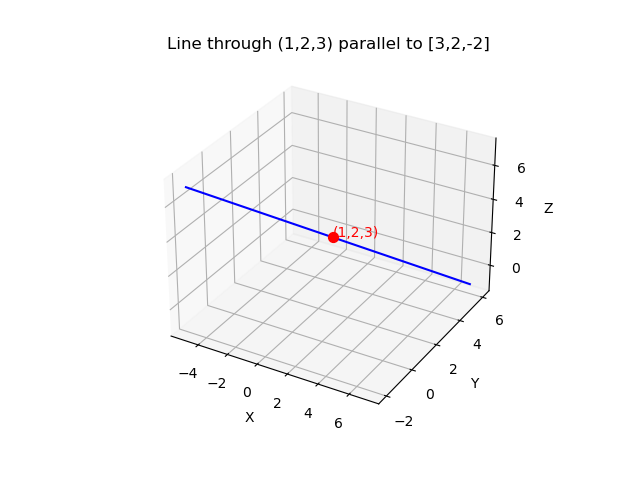
\includegraphics[width=1\columnwidth]{figs/plt.png}
\caption{Line in 3D Plot}
\label{fig:plt}
\end{figure}
\end{frame}

%----------------- C Code -------------------

\begin{frame}[fragile]{C Code (Computations)}
\begin{lstlisting}[language=C]
#include <stdio.h>

void line_point(double kappa, double h[3], double m[3], double out[3]) {
    out[0] = h[0] + kappa * m[0];
    out[1] = h[1] + kappa * m[1];
    out[2] = h[2] + kappa * m[2];
}
\end{lstlisting}
\end{frame}


%----------------- Python Code -------------------
\begin{frame}[fragile]{Python Code (Calling C)}
\begin{lstlisting}[language=Python]
import numpy as np
import ctypes
import matplotlib.pyplot as plt

lib = ctypes.CDLL("./pts.so")

lib.line_point.argtypes = [ctypes.c_double,
                           ctypes.POINTER(ctypes.c_double),
                           ctypes.POINTER(ctypes.c_double),
                           ctypes.POINTER(ctypes.c_double)]

h = np.array([1.0, 2.0, 3.0], dtype=np.float64)
m = np.array([3.0, 2.0, -2.0], dtype=np.float64)
\end{lstlisting}
\end{frame}

\begin{frame}[fragile]{Python Code (cont..)}
\begin{lstlisting}[language=Python]
kappa_values = np.linspace(-2, 2, 100)

points = np.zeros((len(kappa_values), 3), dtype=np.float64)

for i, k in enumerate(kappa_values):
    lib.line_point(ctypes.c_double(k),
                   h.ctypes.data_as(ctypes.POINTER(ctypes.c_double)),
                   m.ctypes.data_as(ctypes.POINTER(ctypes.c_double)),
                   points[i].ctypes.data_as(ctypes.POINTER(ctypes.c_double)))
\end{lstlisting}
\end{frame}

\begin{frame}[fragile]{Python Code (cont..)}
\begin{lstlisting}[language=Python]
fig = plt.figure()
ax = fig.add_subplot(111, projection='3d')
ax.plot(points[:,0], points[:,1], points[:,2], color='blue')
ax.scatter(h[0], h[1], h[2], color='red', s=50)
ax.text(h[0], h[1], h[2], '(1,2,3)', color='red')
ax.set_xlabel('X')
ax.set_ylabel('Y')
ax.set_zlabel('Z')
ax.set_title('3D Line through (1,2,3) parallel to [3,2,-2]')

plt.show()
\end{lstlisting}
\end{frame}

\end{document}